\subsection{Bedienung}
Die Bedienung wurde für eine übersichtliche und schnelle Anwendung einfach gehalten. Auf der Vorderseite hat es drei Tasten und ein Vierzeiliges LCD-Display mit je 16 Charakter für die visuelle Darstellung. Die Tasten sind jeweils Aktiv High am Mikrocontroller angeschlossen mittels einem Taster-Pull-Up-Schaltkreis, zu sehen in Abbildung \ref{fig:SwitchPullUp_Software}. Der Pull-Up Widerstand hat einen Wert von $10k\Omega$, der mit einem Taster auf Erde verbunden wird.

\begin{figure}[h]
	\centering
		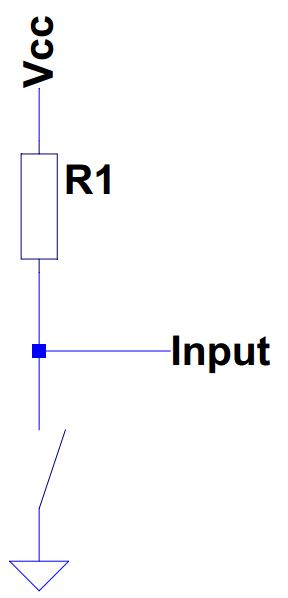
\includegraphics[width=0.15\textwidth]{Taster.jpg}
	\caption{Taster-Pull-Up-Schaltkreis}
	\label{fig:SwitchPullUp_Software}
\end{figure}

Die Taster wurden mit einer Softwarelösung entprellt, ansonsten konnte keine genaue Einstellung der Bestrahlungsstärke erreicht werden, da die Feder im Taster beim Drücken ein undeutliches Signal erzeugt und so ein exaktes und regelmässiges Zählen unmöglich macht. Wird ein Taster betätigt, wird der Widerstand und der Pin des Mikrokontrollers auf Masse verbunden und am Mikrokontroller entsteht ein Low-Zustand, also eine logische Null. Der Taster zustand wird dann mit der Software ausgelesen.

Das Display ist von MIDAS und ist die visuelle Schnittstelle zum Benutzer. Der LCD ist im vier Bit Modus an den Mikrocontroller angeschlossen. Für VisualSun wurden nur die Kontakte DB0 bis DB3 benötigt. Die restlichen Kontakte DB4 bis DB7 und der Lesen-Schreiben-Anschluss (Read-Write-Pin) wurden auf Erde verbunden. Der LCD wird mit 5 Volt über den Mikrocontroller versorgt. Das genaue Anschlussschema  ist in Abbildung \ref{fig:AnschlussSchema} ersichtlich.

\begin{figure}[h]
	\centering
		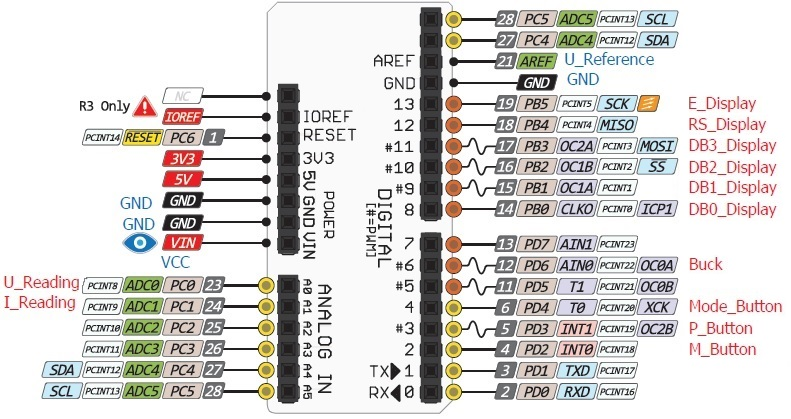
\includegraphics[width=0.8\textwidth]{Anschlussschema.jpg}
	\caption{Anschlussschema für LCD und Tasten am Arduino UNO}
	\label{fig:AnschlussSchema}
\end{figure}